\section{Results}

\begin{frame}{MSD vs. PCA - Baseline set length ($b$)}

    Here we observe the effect of the baseline set length $b$ on the accuracy of the two methods.

    \begin{figure}[H]
        \centering
        \only<1>{
            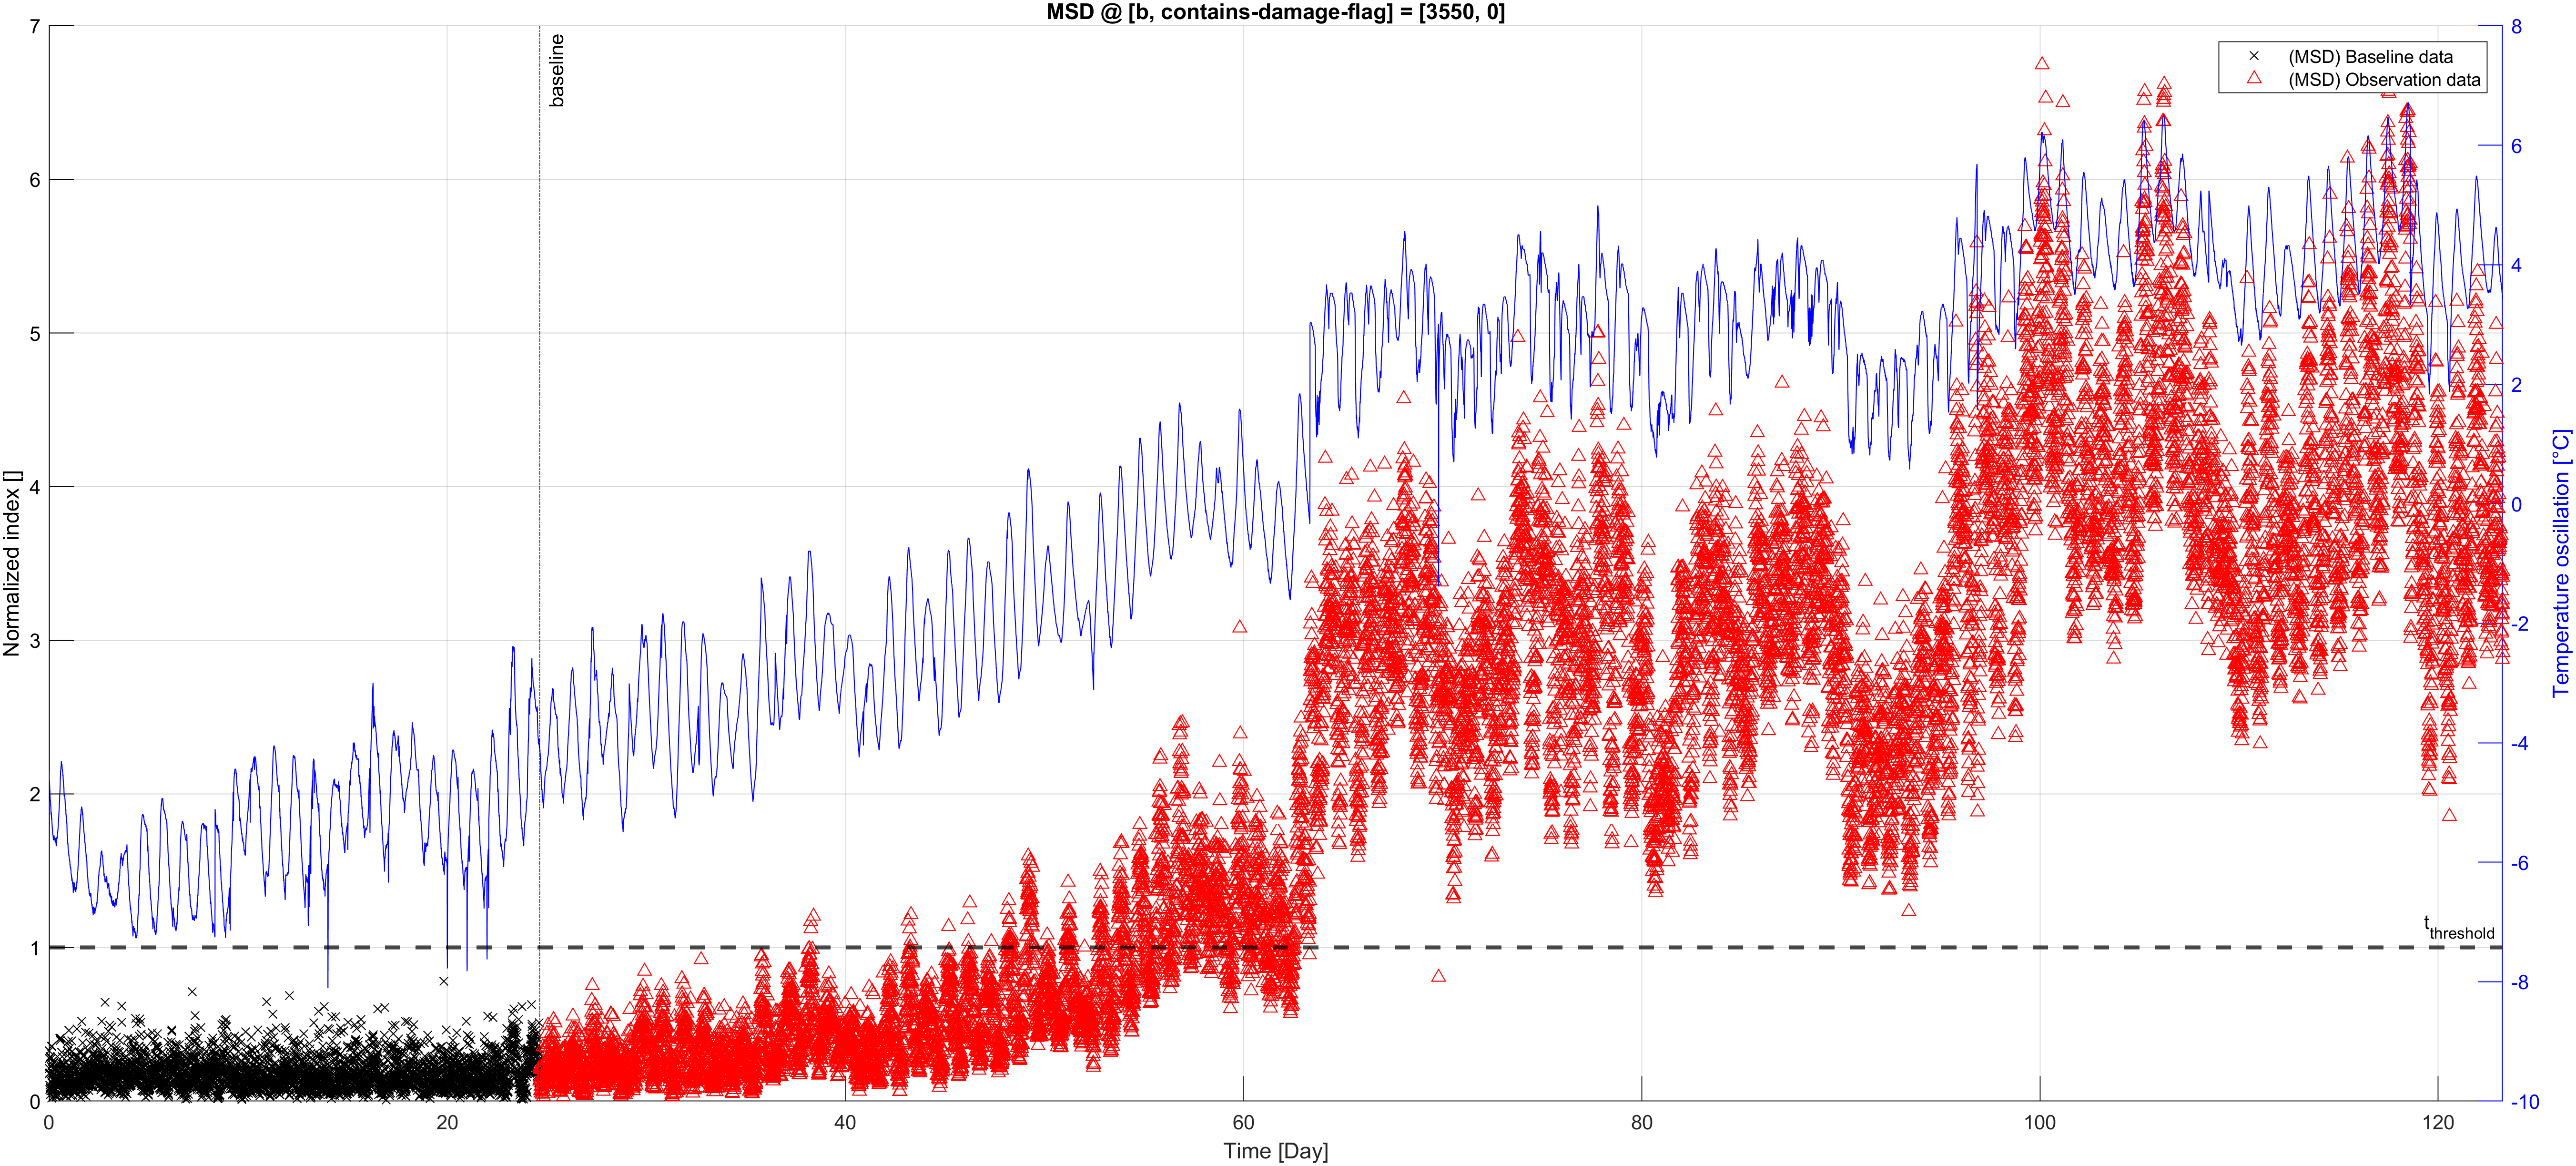
\includegraphics[width=0.9\textwidth]{img/Baseline/MSD_Baseline_3550.png}
            \caption{MSD method considering $b = 3550$}
        }
        \only<2>{
            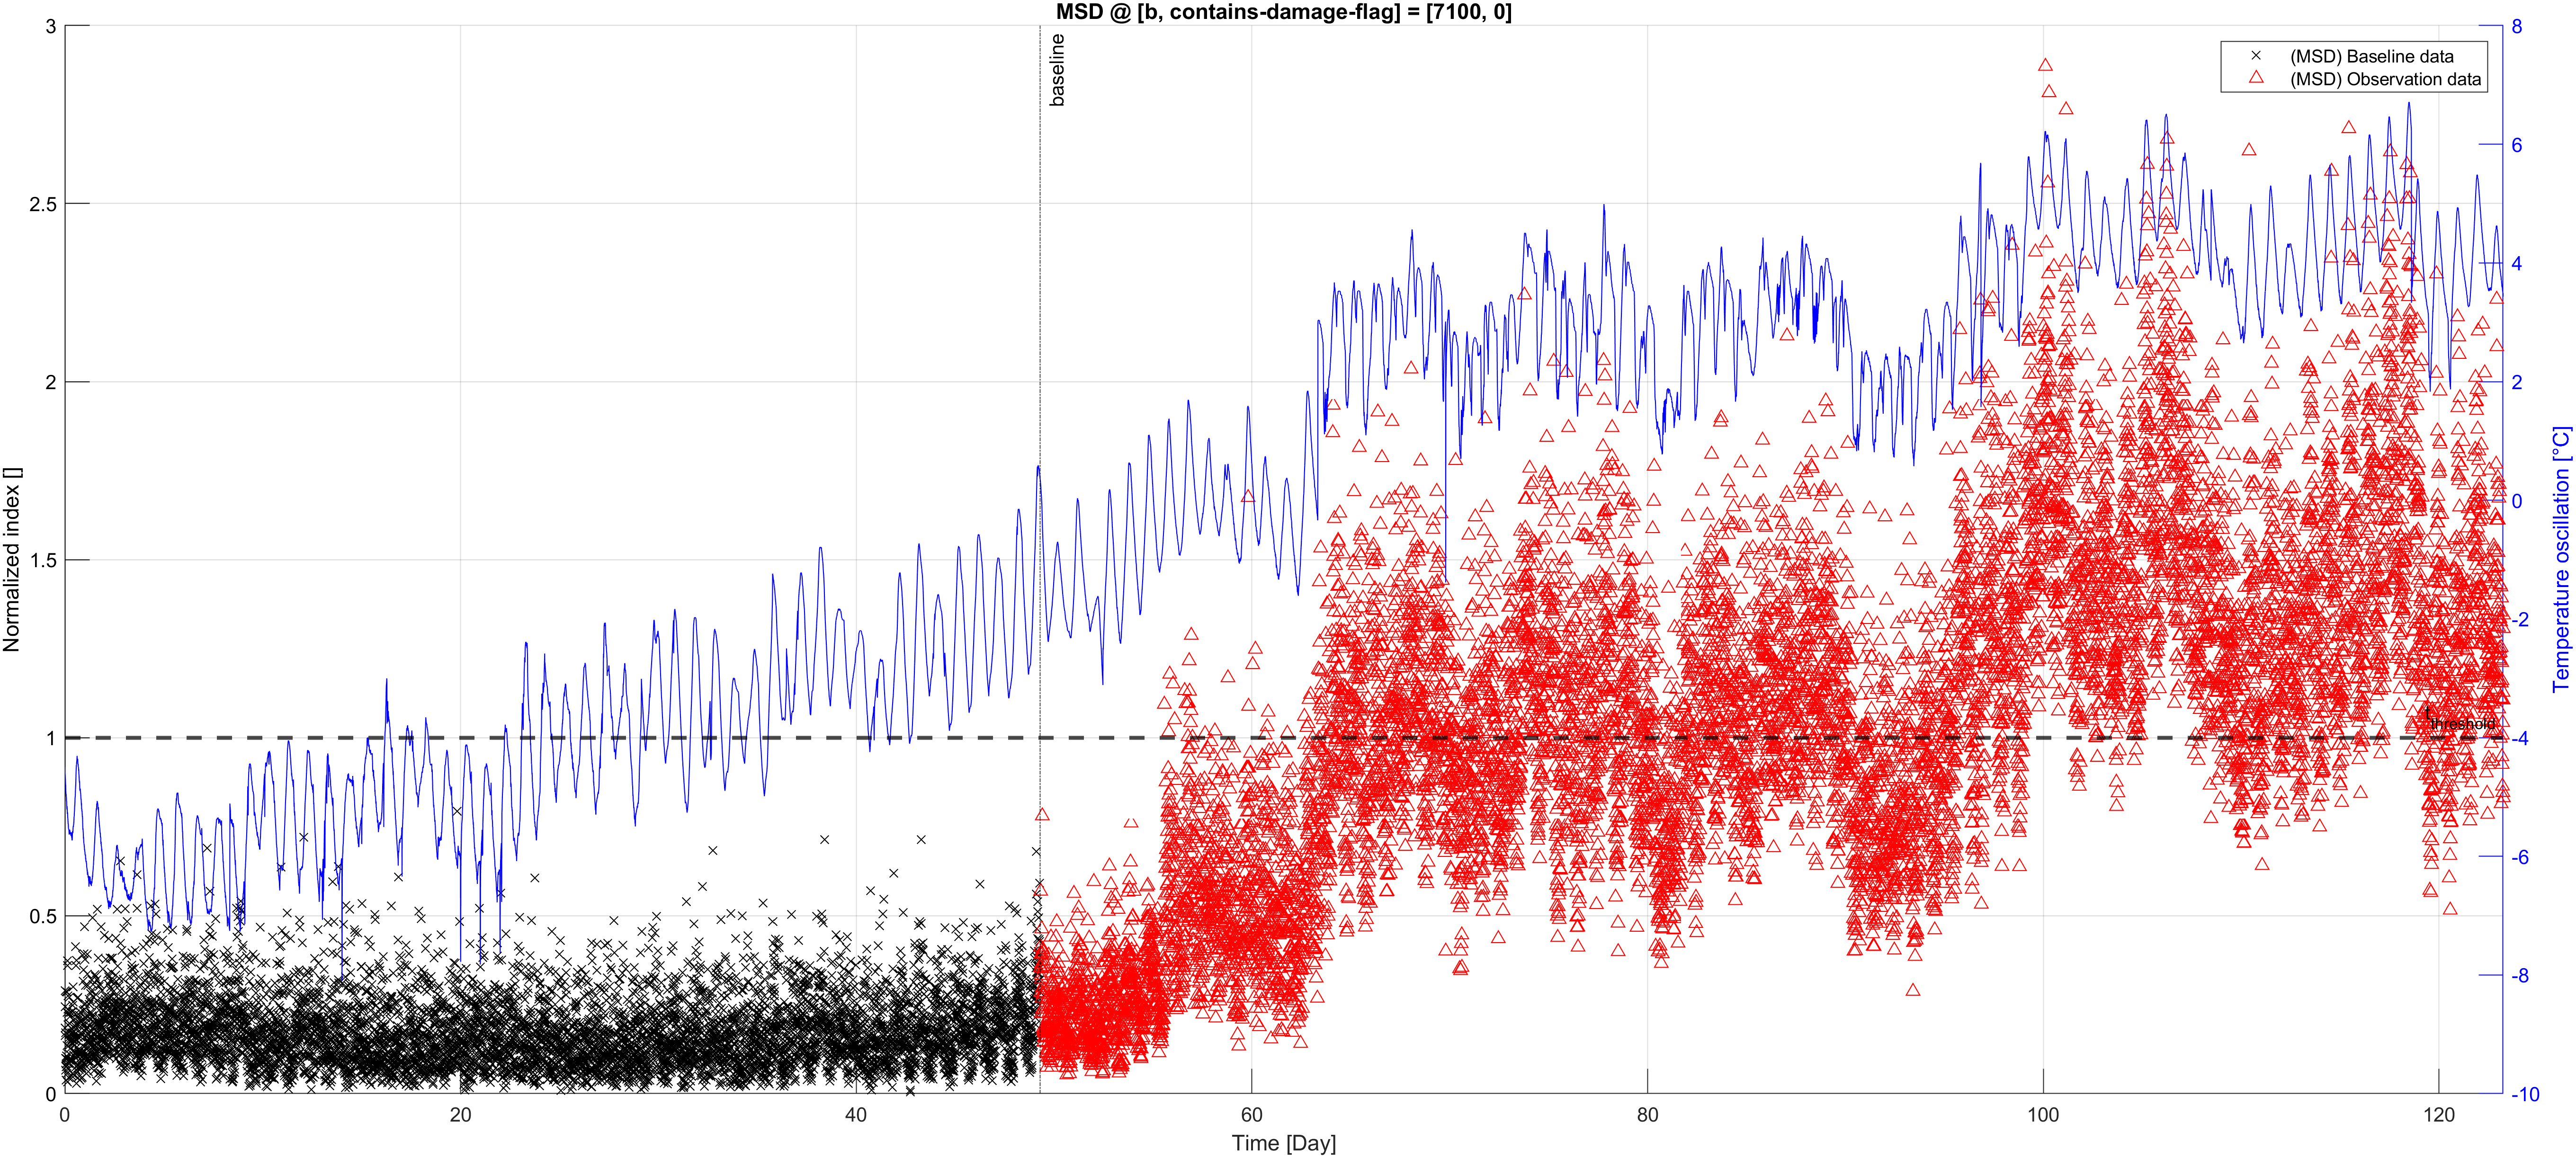
\includegraphics[width=0.9\textwidth]{img/Baseline/MSD_Baseline_7100.png}
            \caption{MSD method considering $b = 7000$}
        }
        \only<3>{
            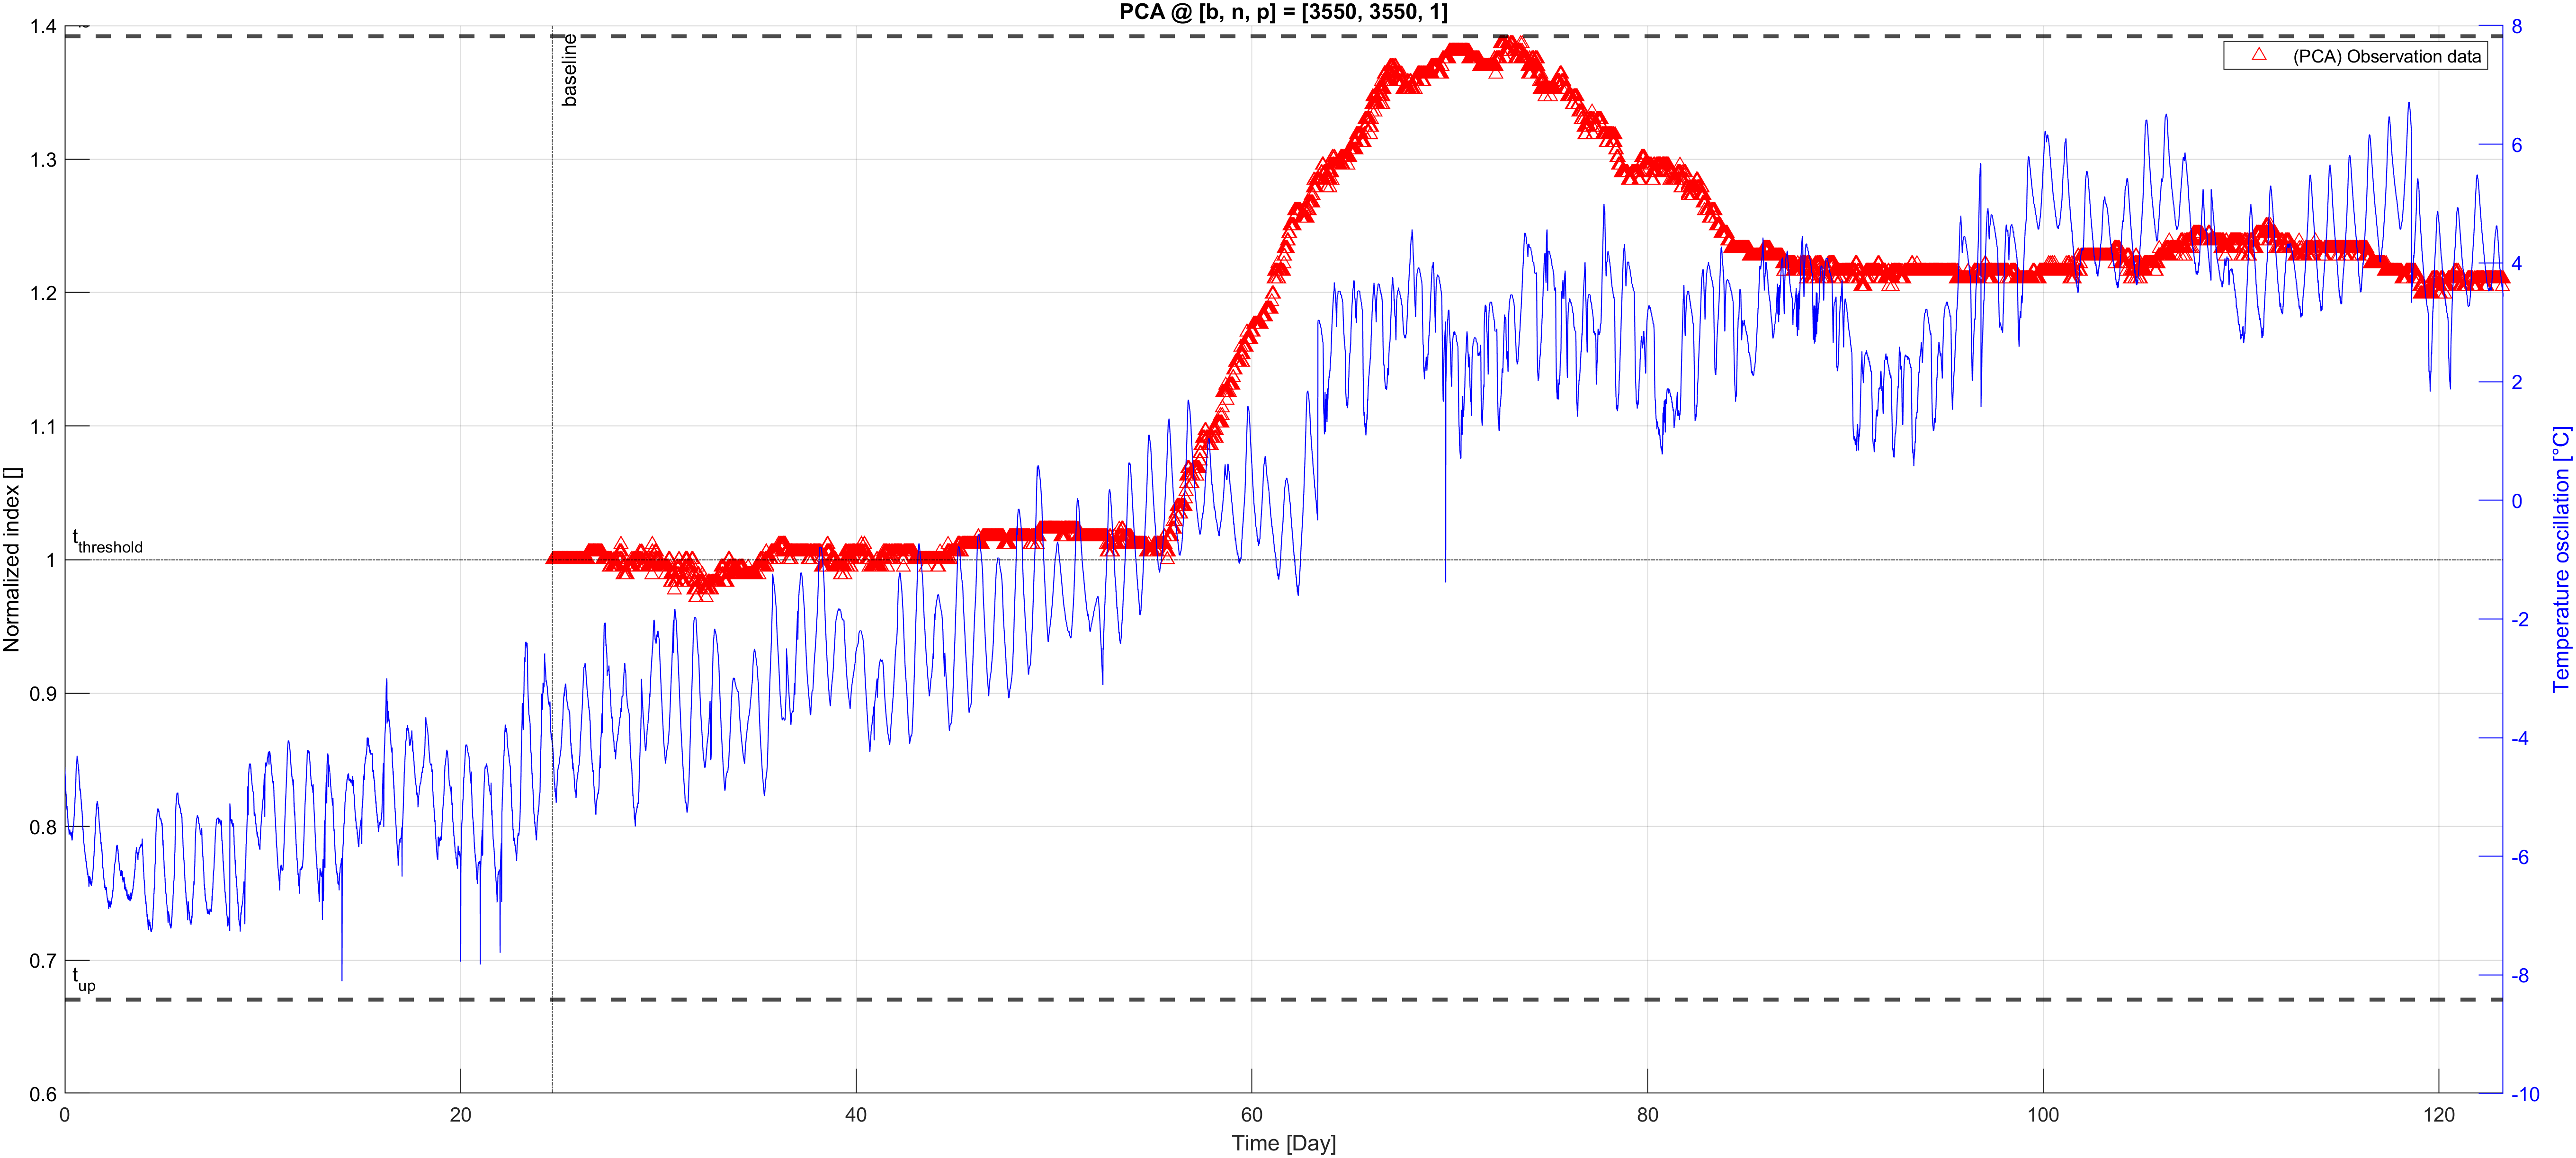
\includegraphics[width=0.9\textwidth]{img/Baseline/PCA_Baseline_3550.png}
            \caption{PCA method considering $b = n = 3550$}
        }
        \only<4>{
            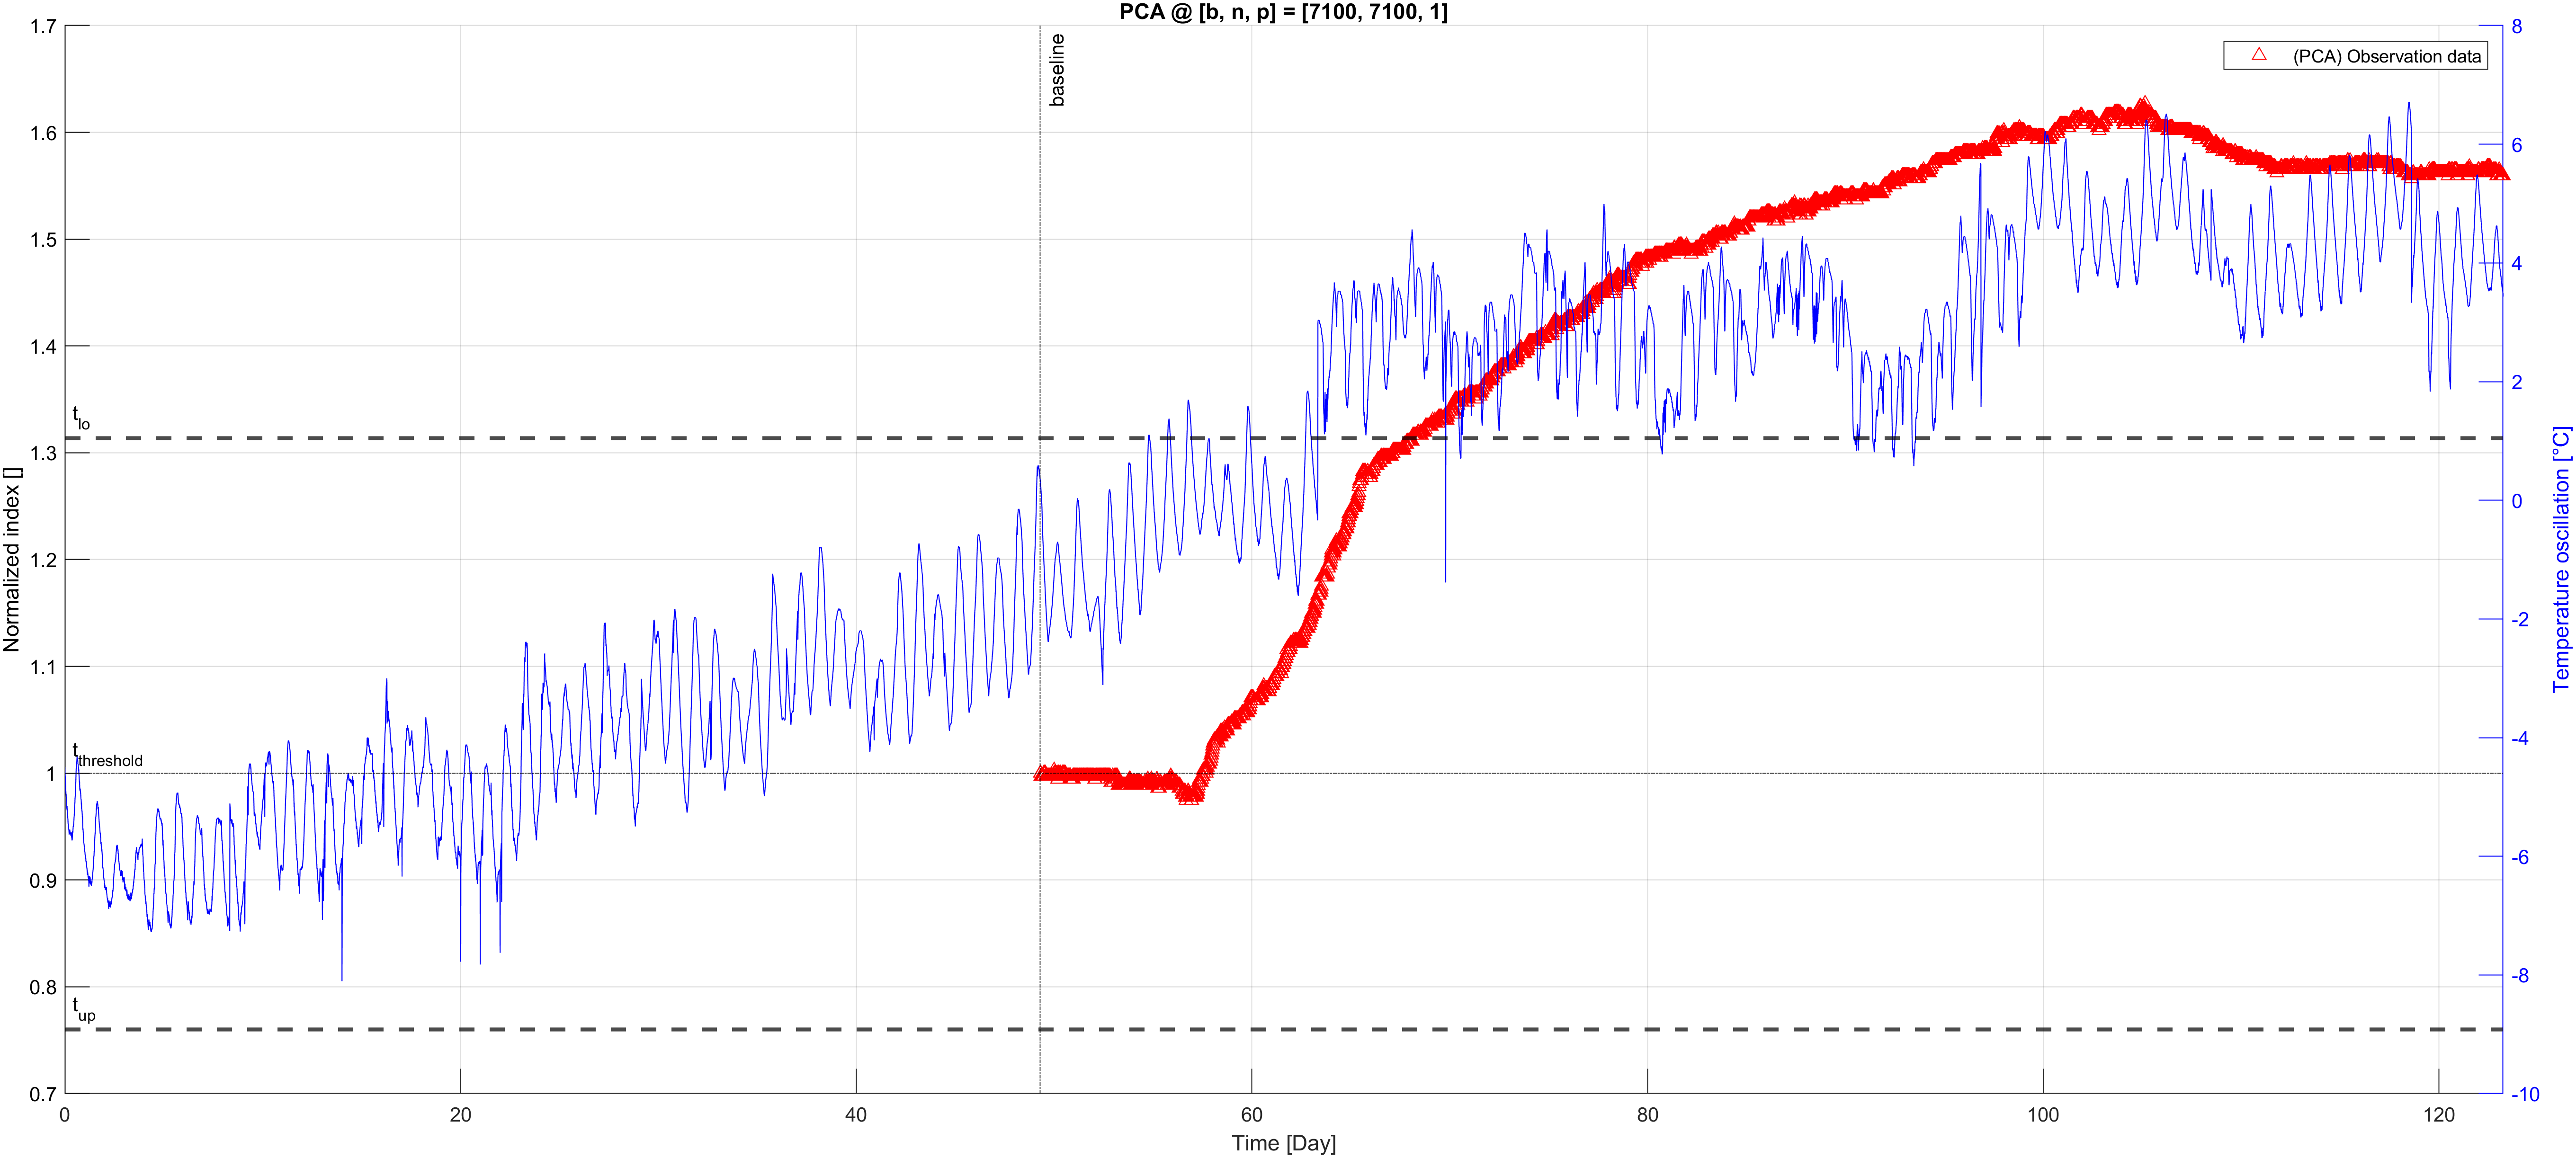
\includegraphics[width=0.9\textwidth]{img/Baseline/PCA_Baseline_7100.png}
            \caption{PCA method considering $b = n = 7000$}
        }
    \end{figure}

    \vspace{-9pt}

    The MSD method is highly sensitive to $b$ and if the baseline set doesn't contain a complete set of environmental conditions, it may lead to false positives/negative.

\end{frame}



\begin{frame}{PCA - Observation window length ($n$)}

    A key difference between the MSD and PCA methods is that MSD compute the index for each observation record, while PCA computes the index for a set of records with length $n$.

    \begin{figure}[H]
        \centering
        \only<1>{
            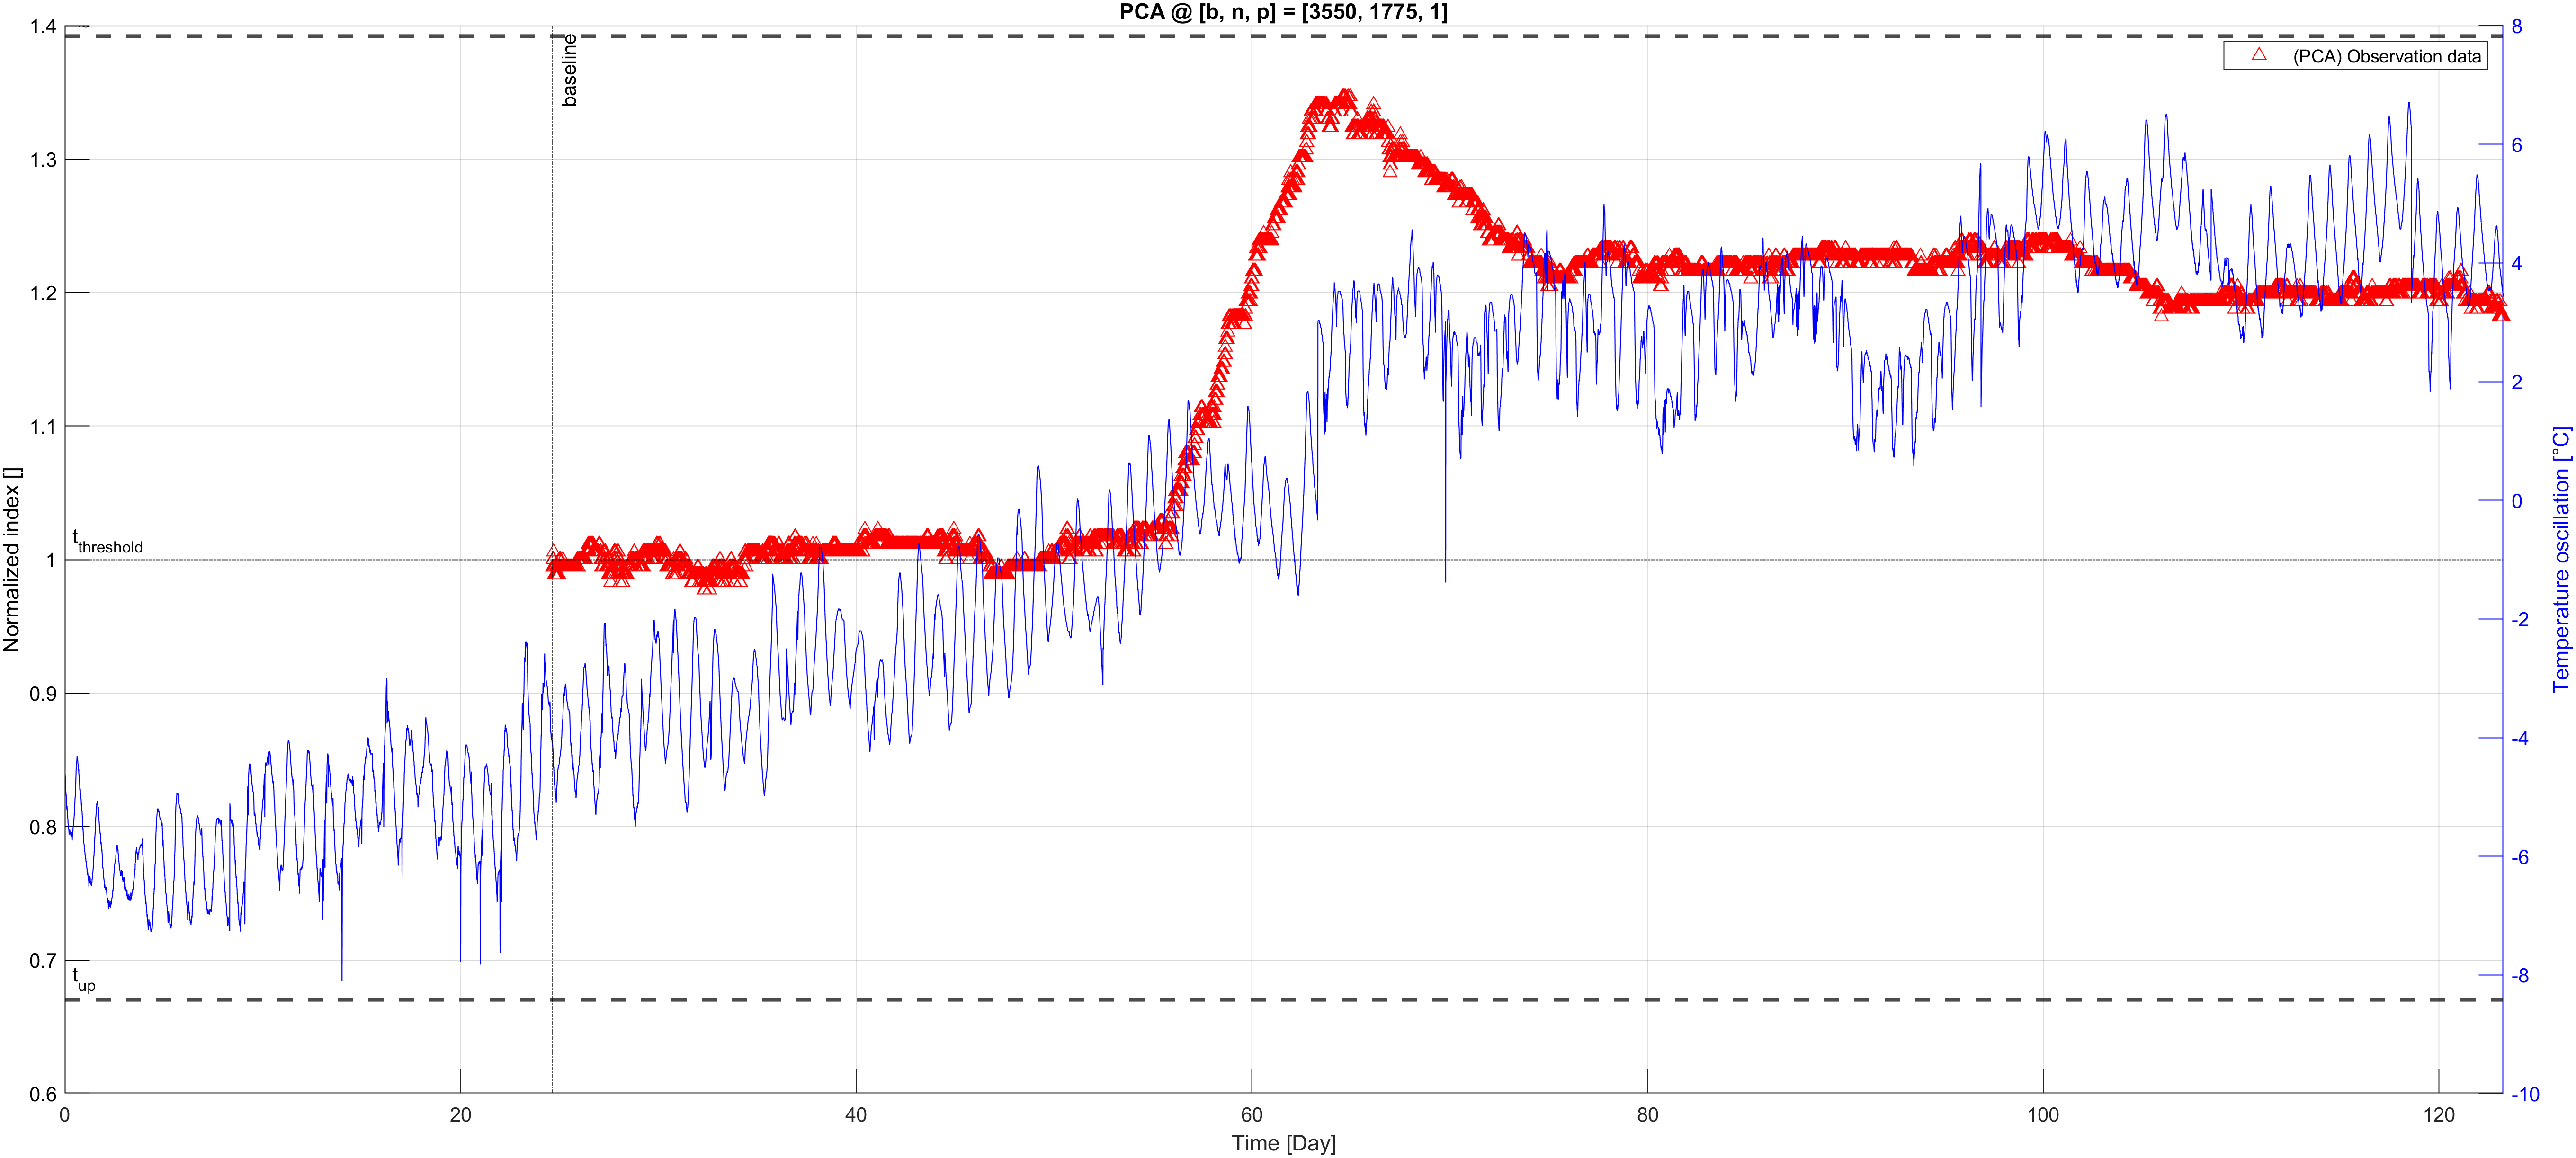
\includegraphics[width=0.9\textwidth]{img/Window/PCA_Window_1775.png}
            \caption{PCA method considering $b = 3550$ \& $n = 1775$}
        }
        \only<2>{
            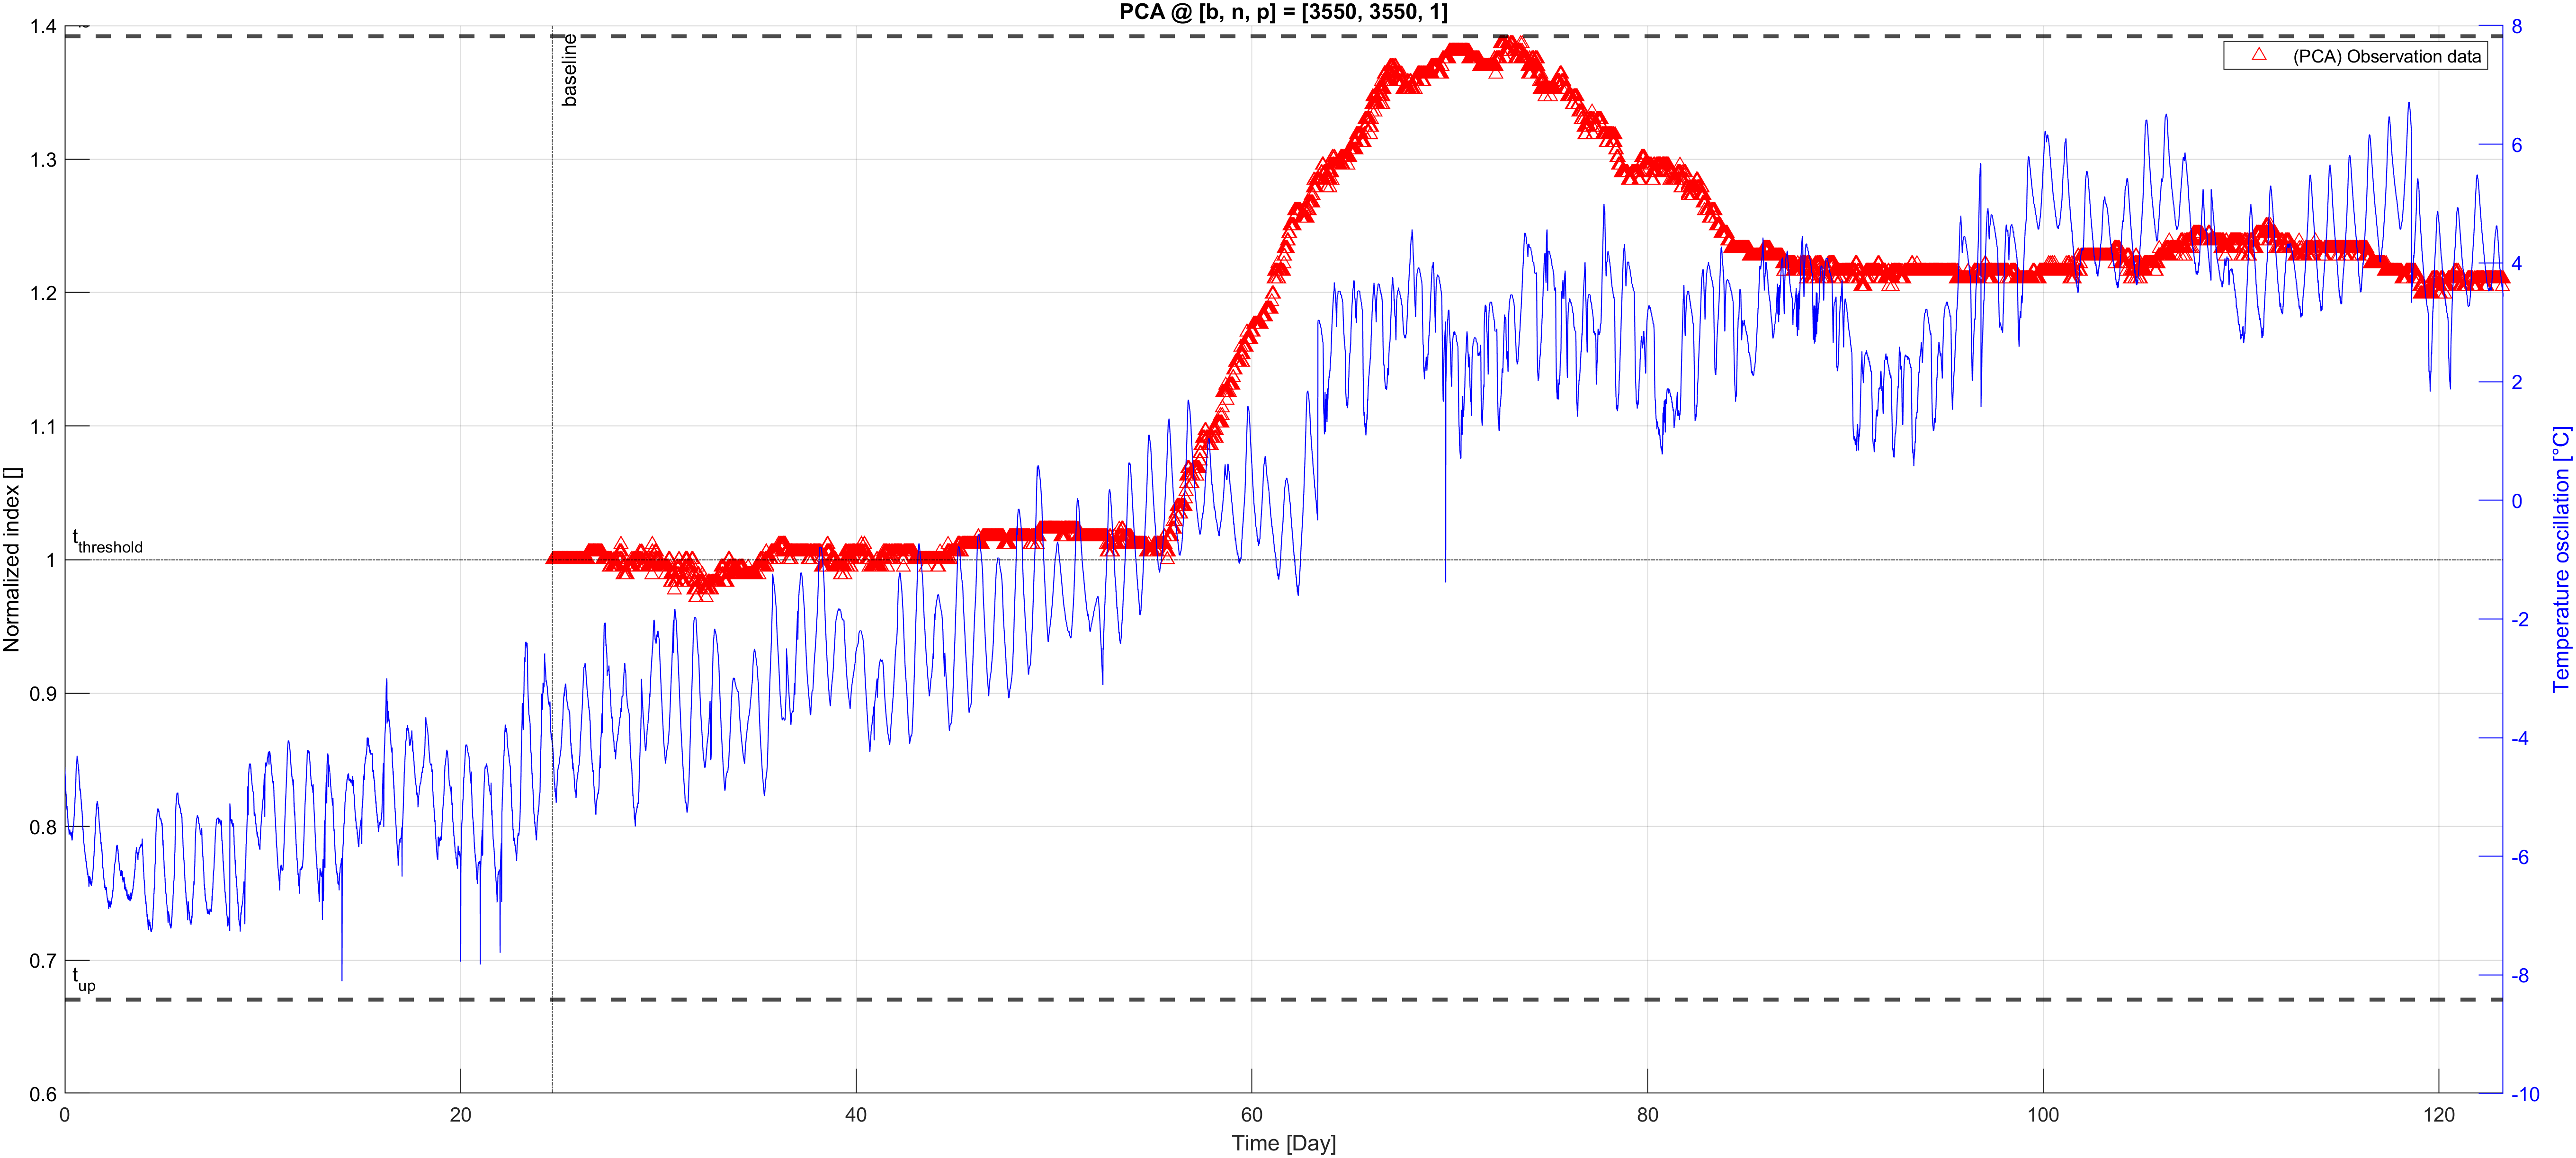
\includegraphics[width=0.9\textwidth]{img/Window/PCA_Window_3550.png}
            \caption{PCA method considering $b = 3550$ \& $n = 3550$}
        }
        \only<3>{
            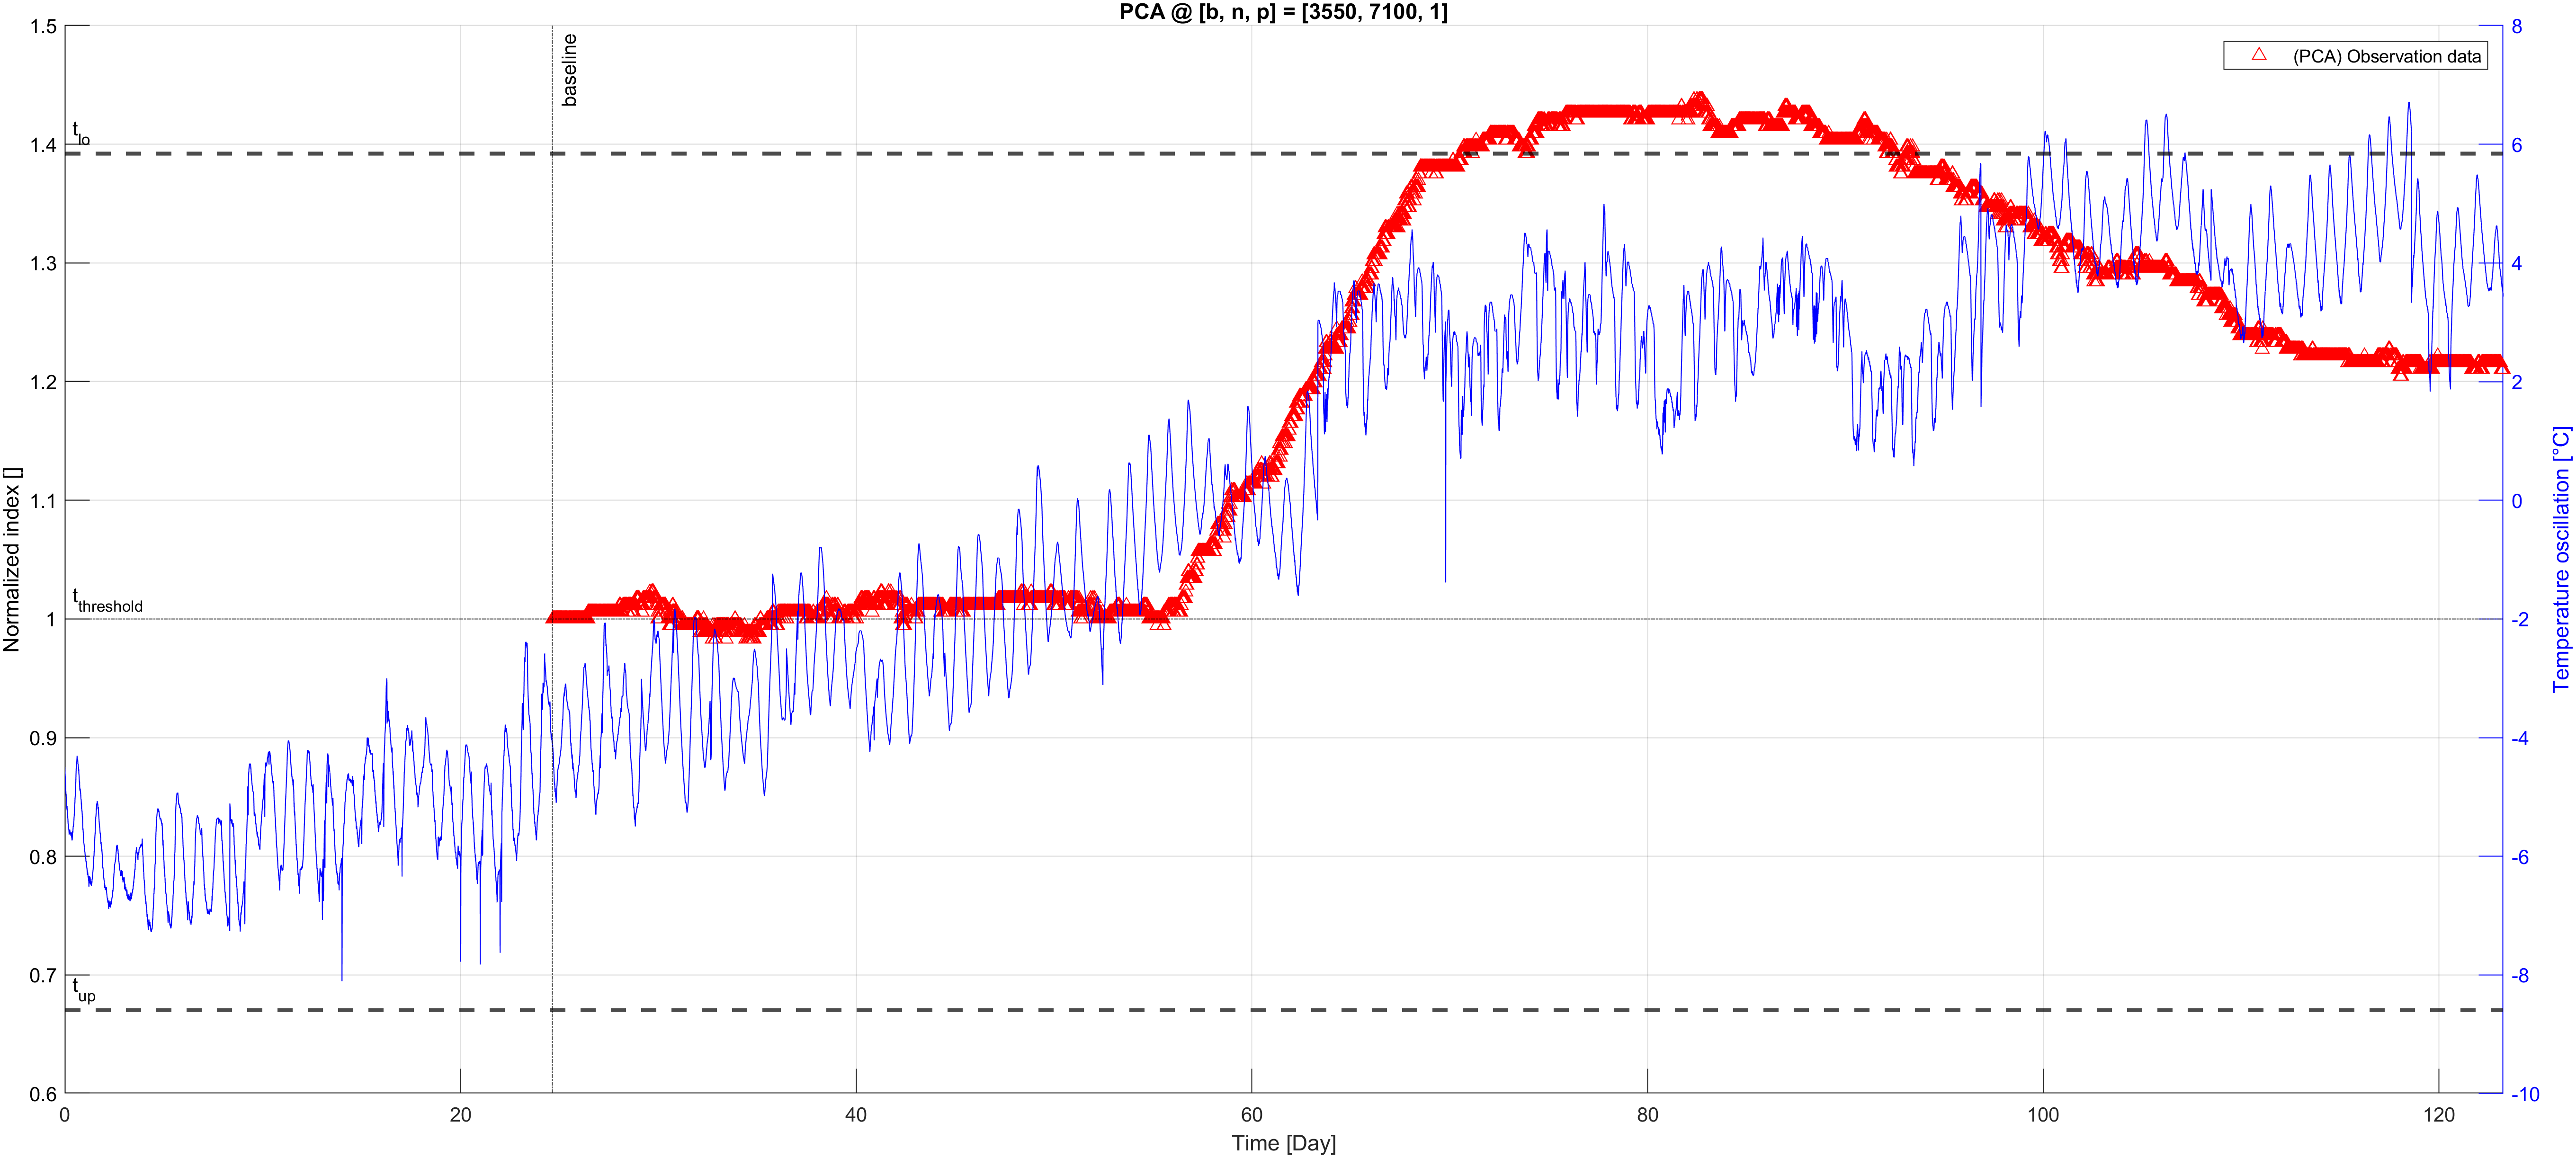
\includegraphics[width=0.9\textwidth]{img/Window/PCA_Window_7100.png}
            \caption{PCA method considering $b = 3550$ \& $n = 7100$}
        }
        \only<4>{
            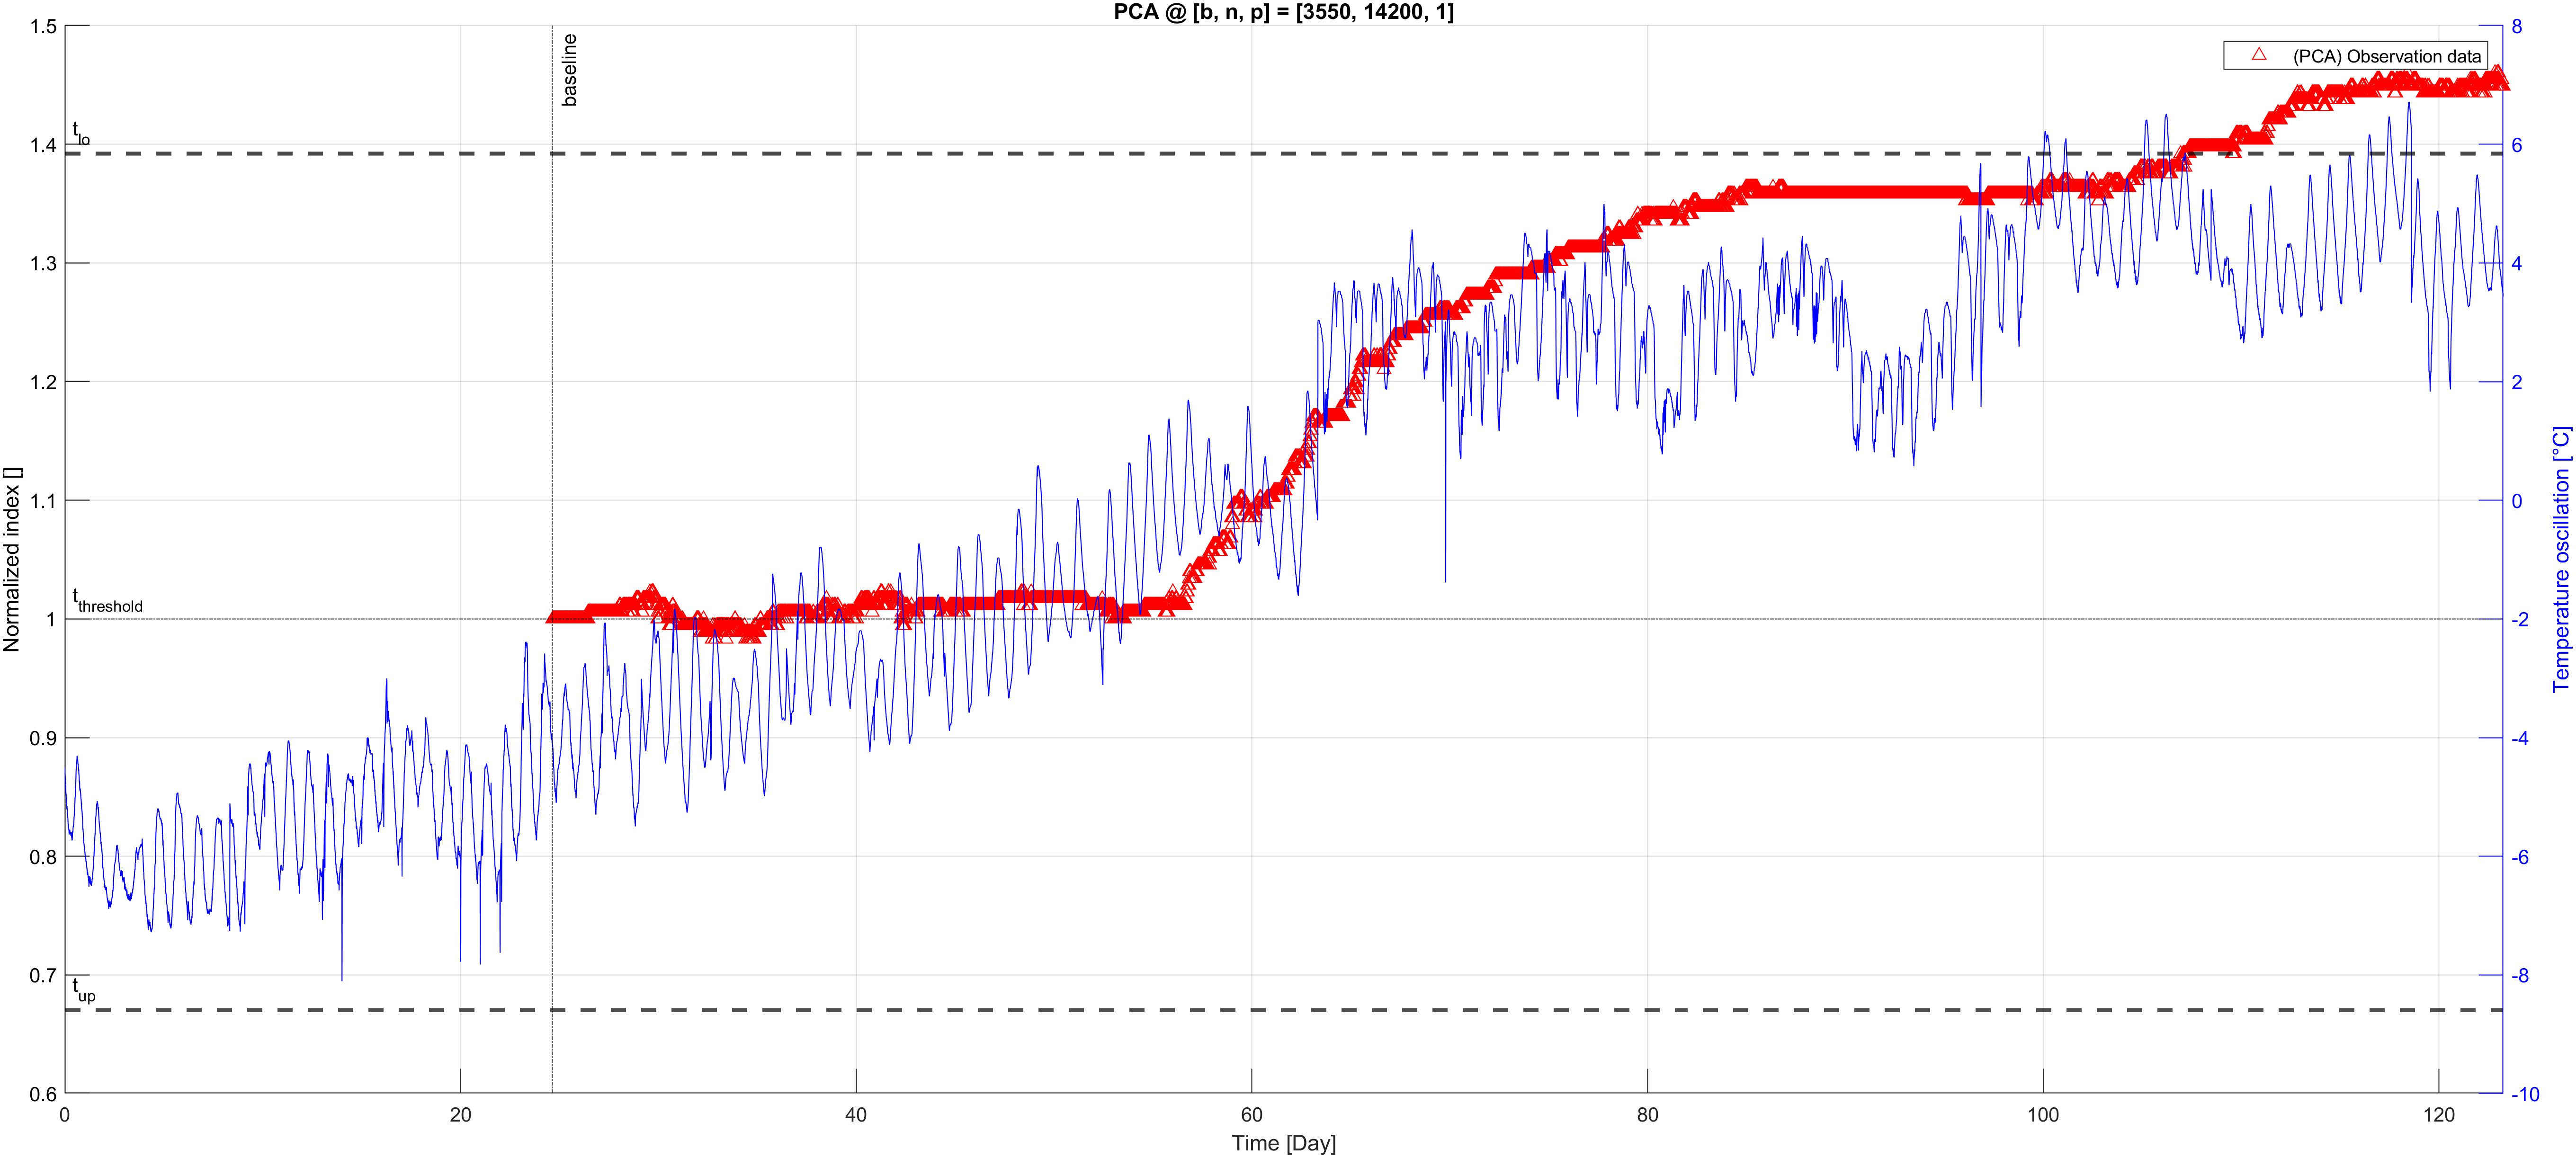
\includegraphics[width=0.9\textwidth]{img/Window/PCA_Window_14200.png}
            \caption{PCA method considering $b = 3550$ \& $n = 14200$}
        }
    \end{figure}

    \vspace{-9pt}

    It's clear how $n$ affect the reactivity of the PCA method to detect outliers.
    In particular, the higher $n$, the longer the transient time before the detection of the feature.

\end{frame}